\documentclass{beamer}
\usepackage{lmodern}
\usepackage[T1]{fontenc}
\beamertemplatenavigationsymbolsempty
\title[]{Visualisierung komplexer Datenstrukturen}
\author[]{Yannick Miguel, Kjell Noack, Florian Schürenberg, Jacqueline Link}
\date[27.02.2024]{27. Februar 2024}
\setbeamercovered{transparent}
\usepackage[backend=biber]{biblatex}
\usepackage{graphicx}
\usepackage{booktabs}
\usetheme{Boadilla}
%\definecolor{myOrange}{rgb}{0.110,0.199,0.45}                   
%\usecolortheme[RGB={110,199,45}]{structure}  
\useinnertheme{rounded}
\usepackage{tikz}
\setbeamertemplate{caption}[numbered]
\addbibresource{Quellen.bib}

\begin{document} 
	\begin{frame}
		\maketitle
	\end{frame}        
	\begin{frame}
		\frametitle{Inhaltsverzeichnis}
		\tableofcontents
	\end{frame}
	\addtocounter{framenumber}{-1}
	\section{Gründe für Betriebsverlassung}
	\begin{frame}
		\frametitle{Gründe für Betriebsverlassung}
		\begin{figure}[htbp]
			\centering
			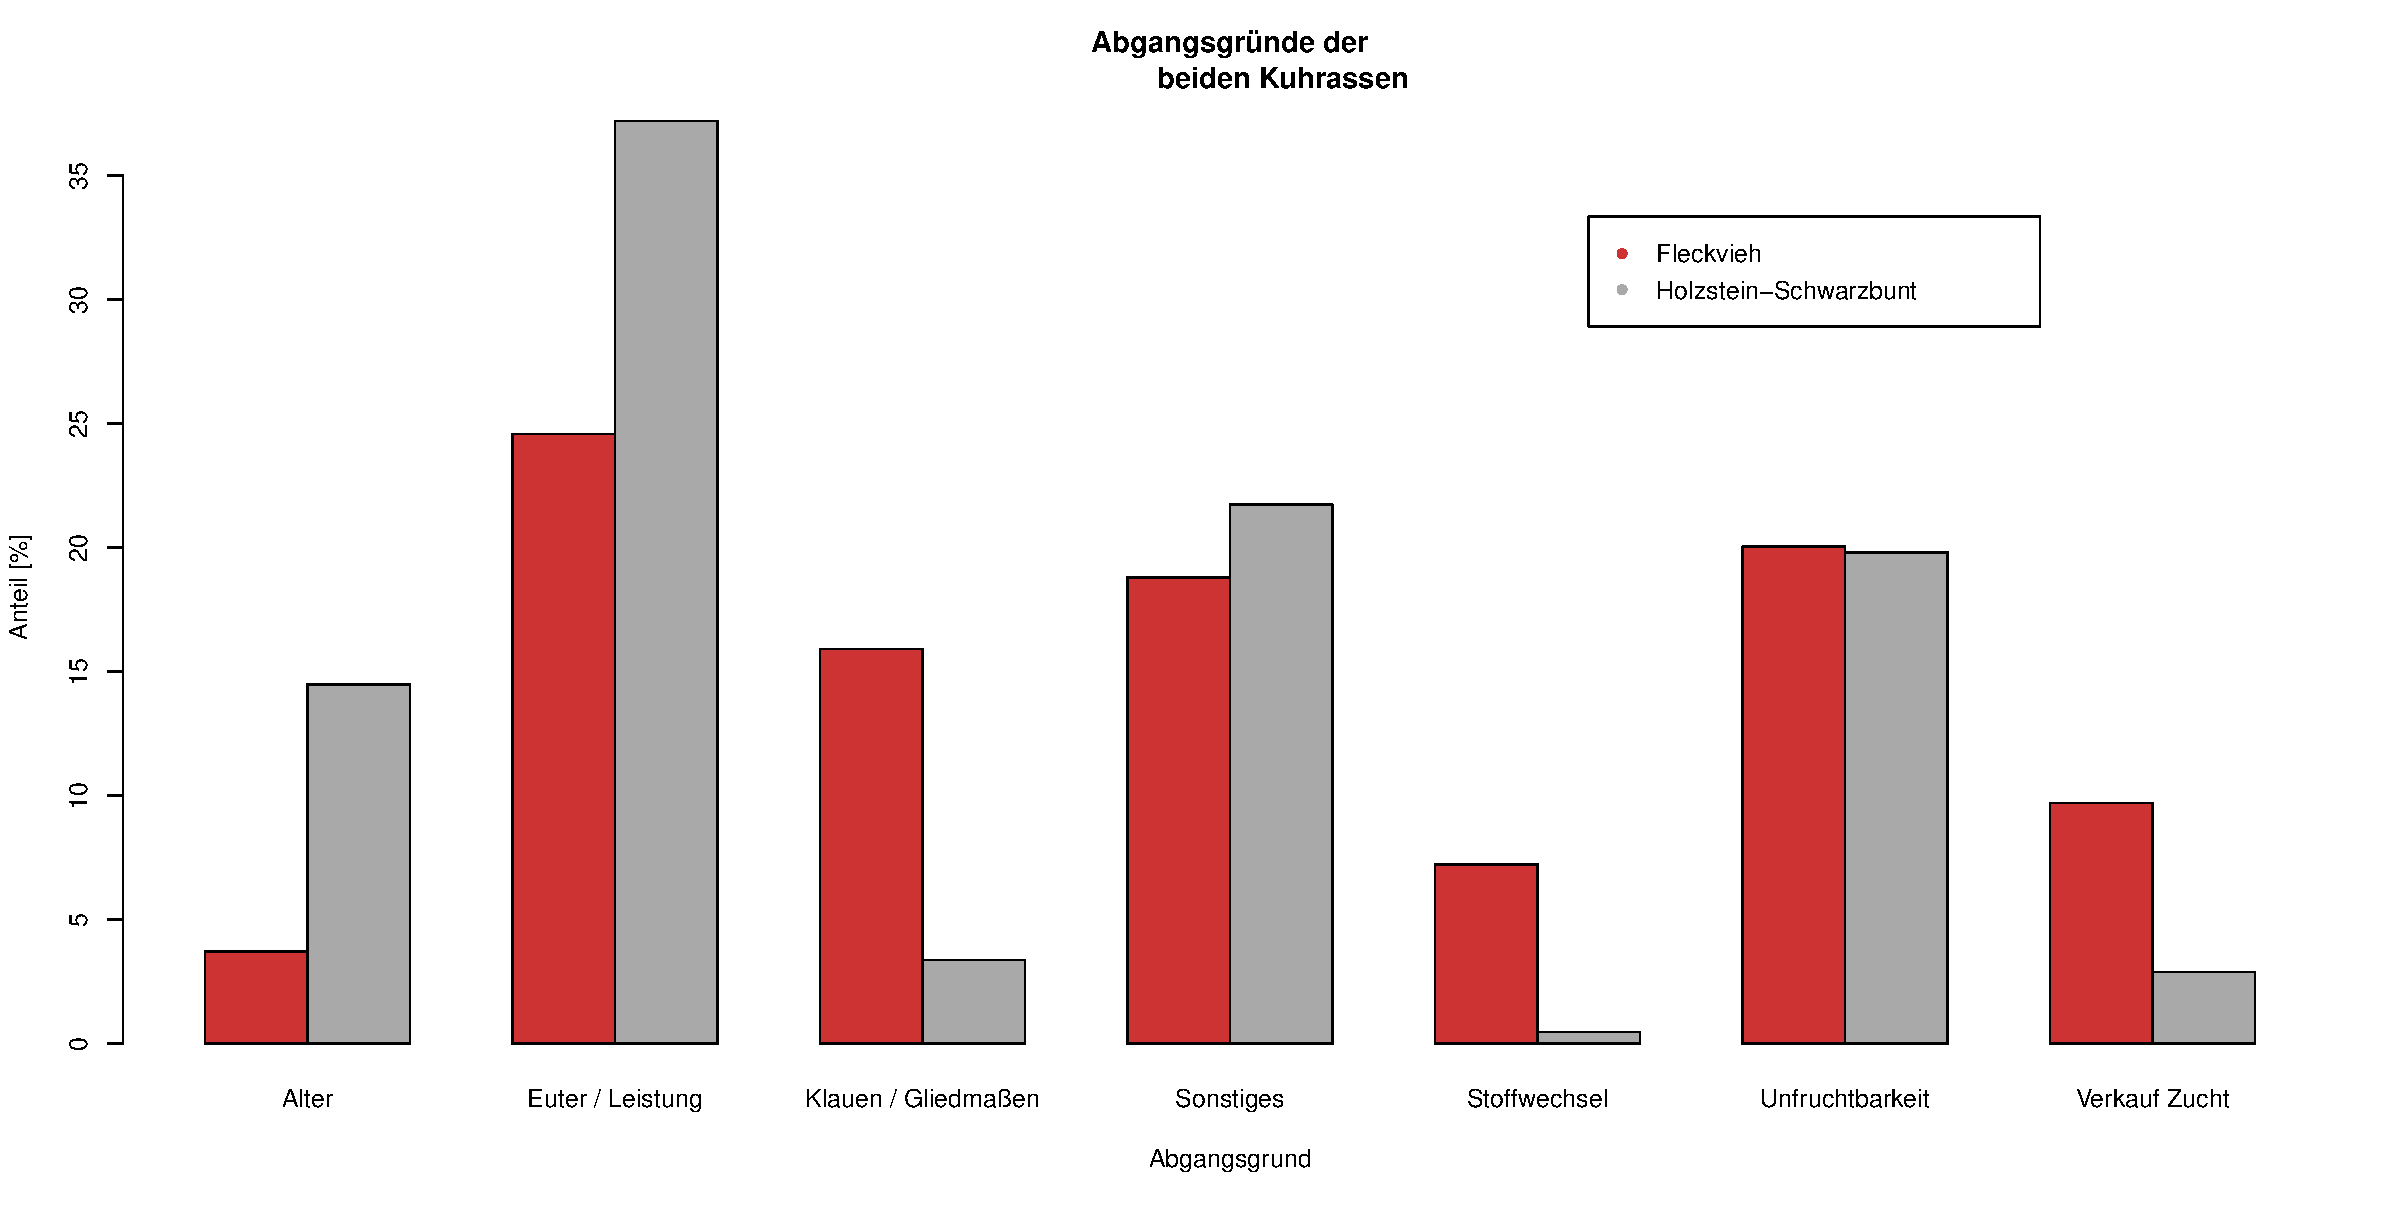
\includegraphics[scale = 0.32]{abgang.pdf}
			\caption{Säulendiagramme zu den Abgangsgründen der beiden Kuhrassen}
		\end{figure}
	\end{frame}
	
	\section{Laktationseinflüsse}
	\begin{frame}
		\frametitle{Laktationseinflüsse}
		\begin{figure}[htbp]
			\centering
			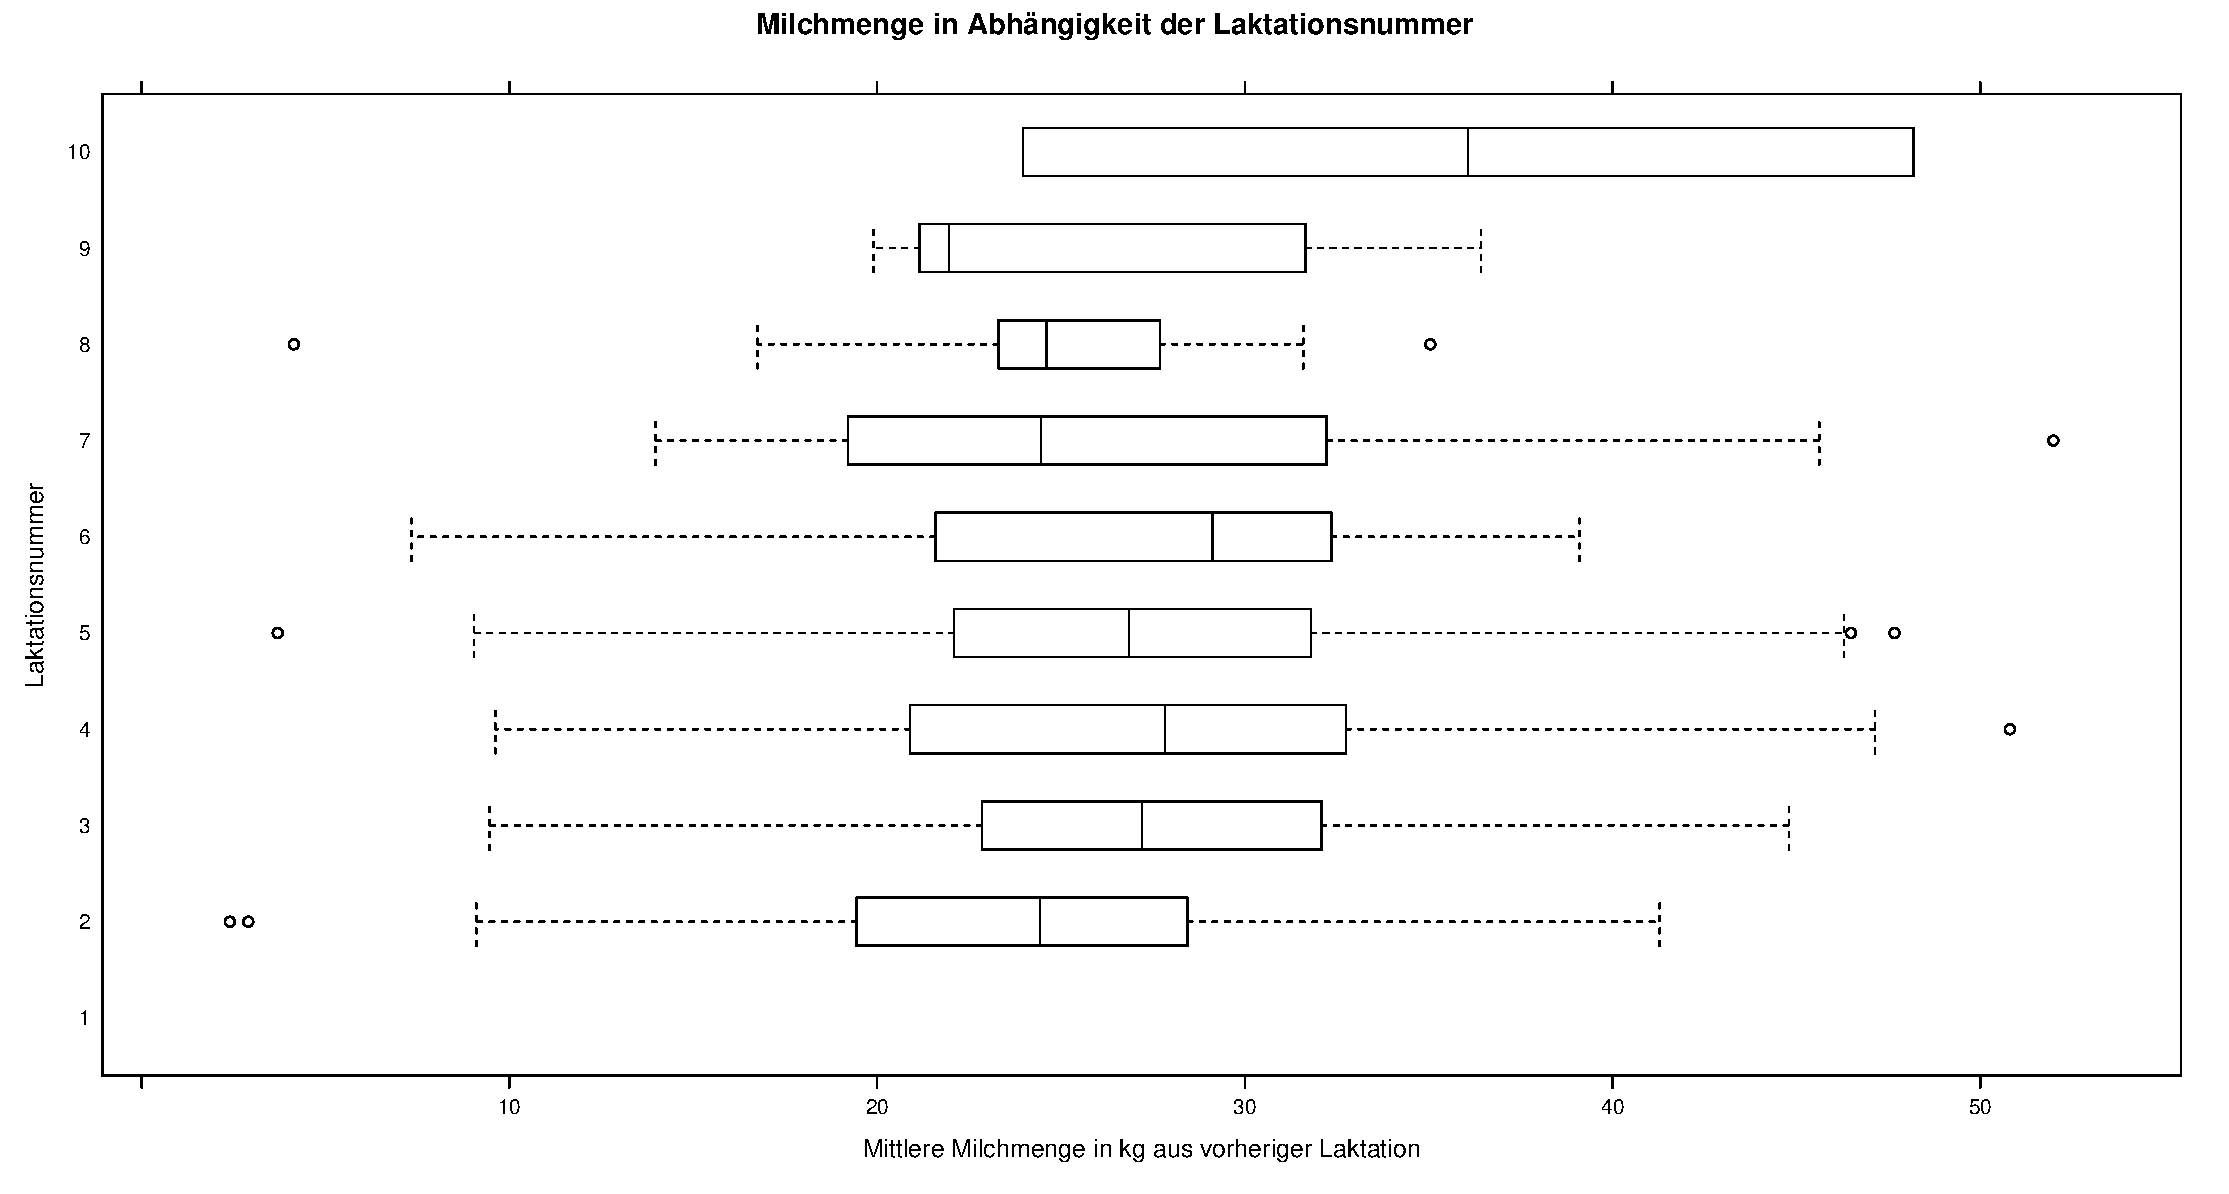
\includegraphics[scale = 0.333]{lattice.pdf}
			\vspace{-0.6cm}
			\caption{Boxplots zur Gegenüberstellung der Milchmenge und der aktuellen Laktationsnummer}
		\end{figure}
	\end{frame}

    	\section{Milchmenge und Gewicht}
	\begin{frame}
		\frametitle{Milchmenge und Gewicht}
		\begin{figure}[h]
			\centering
			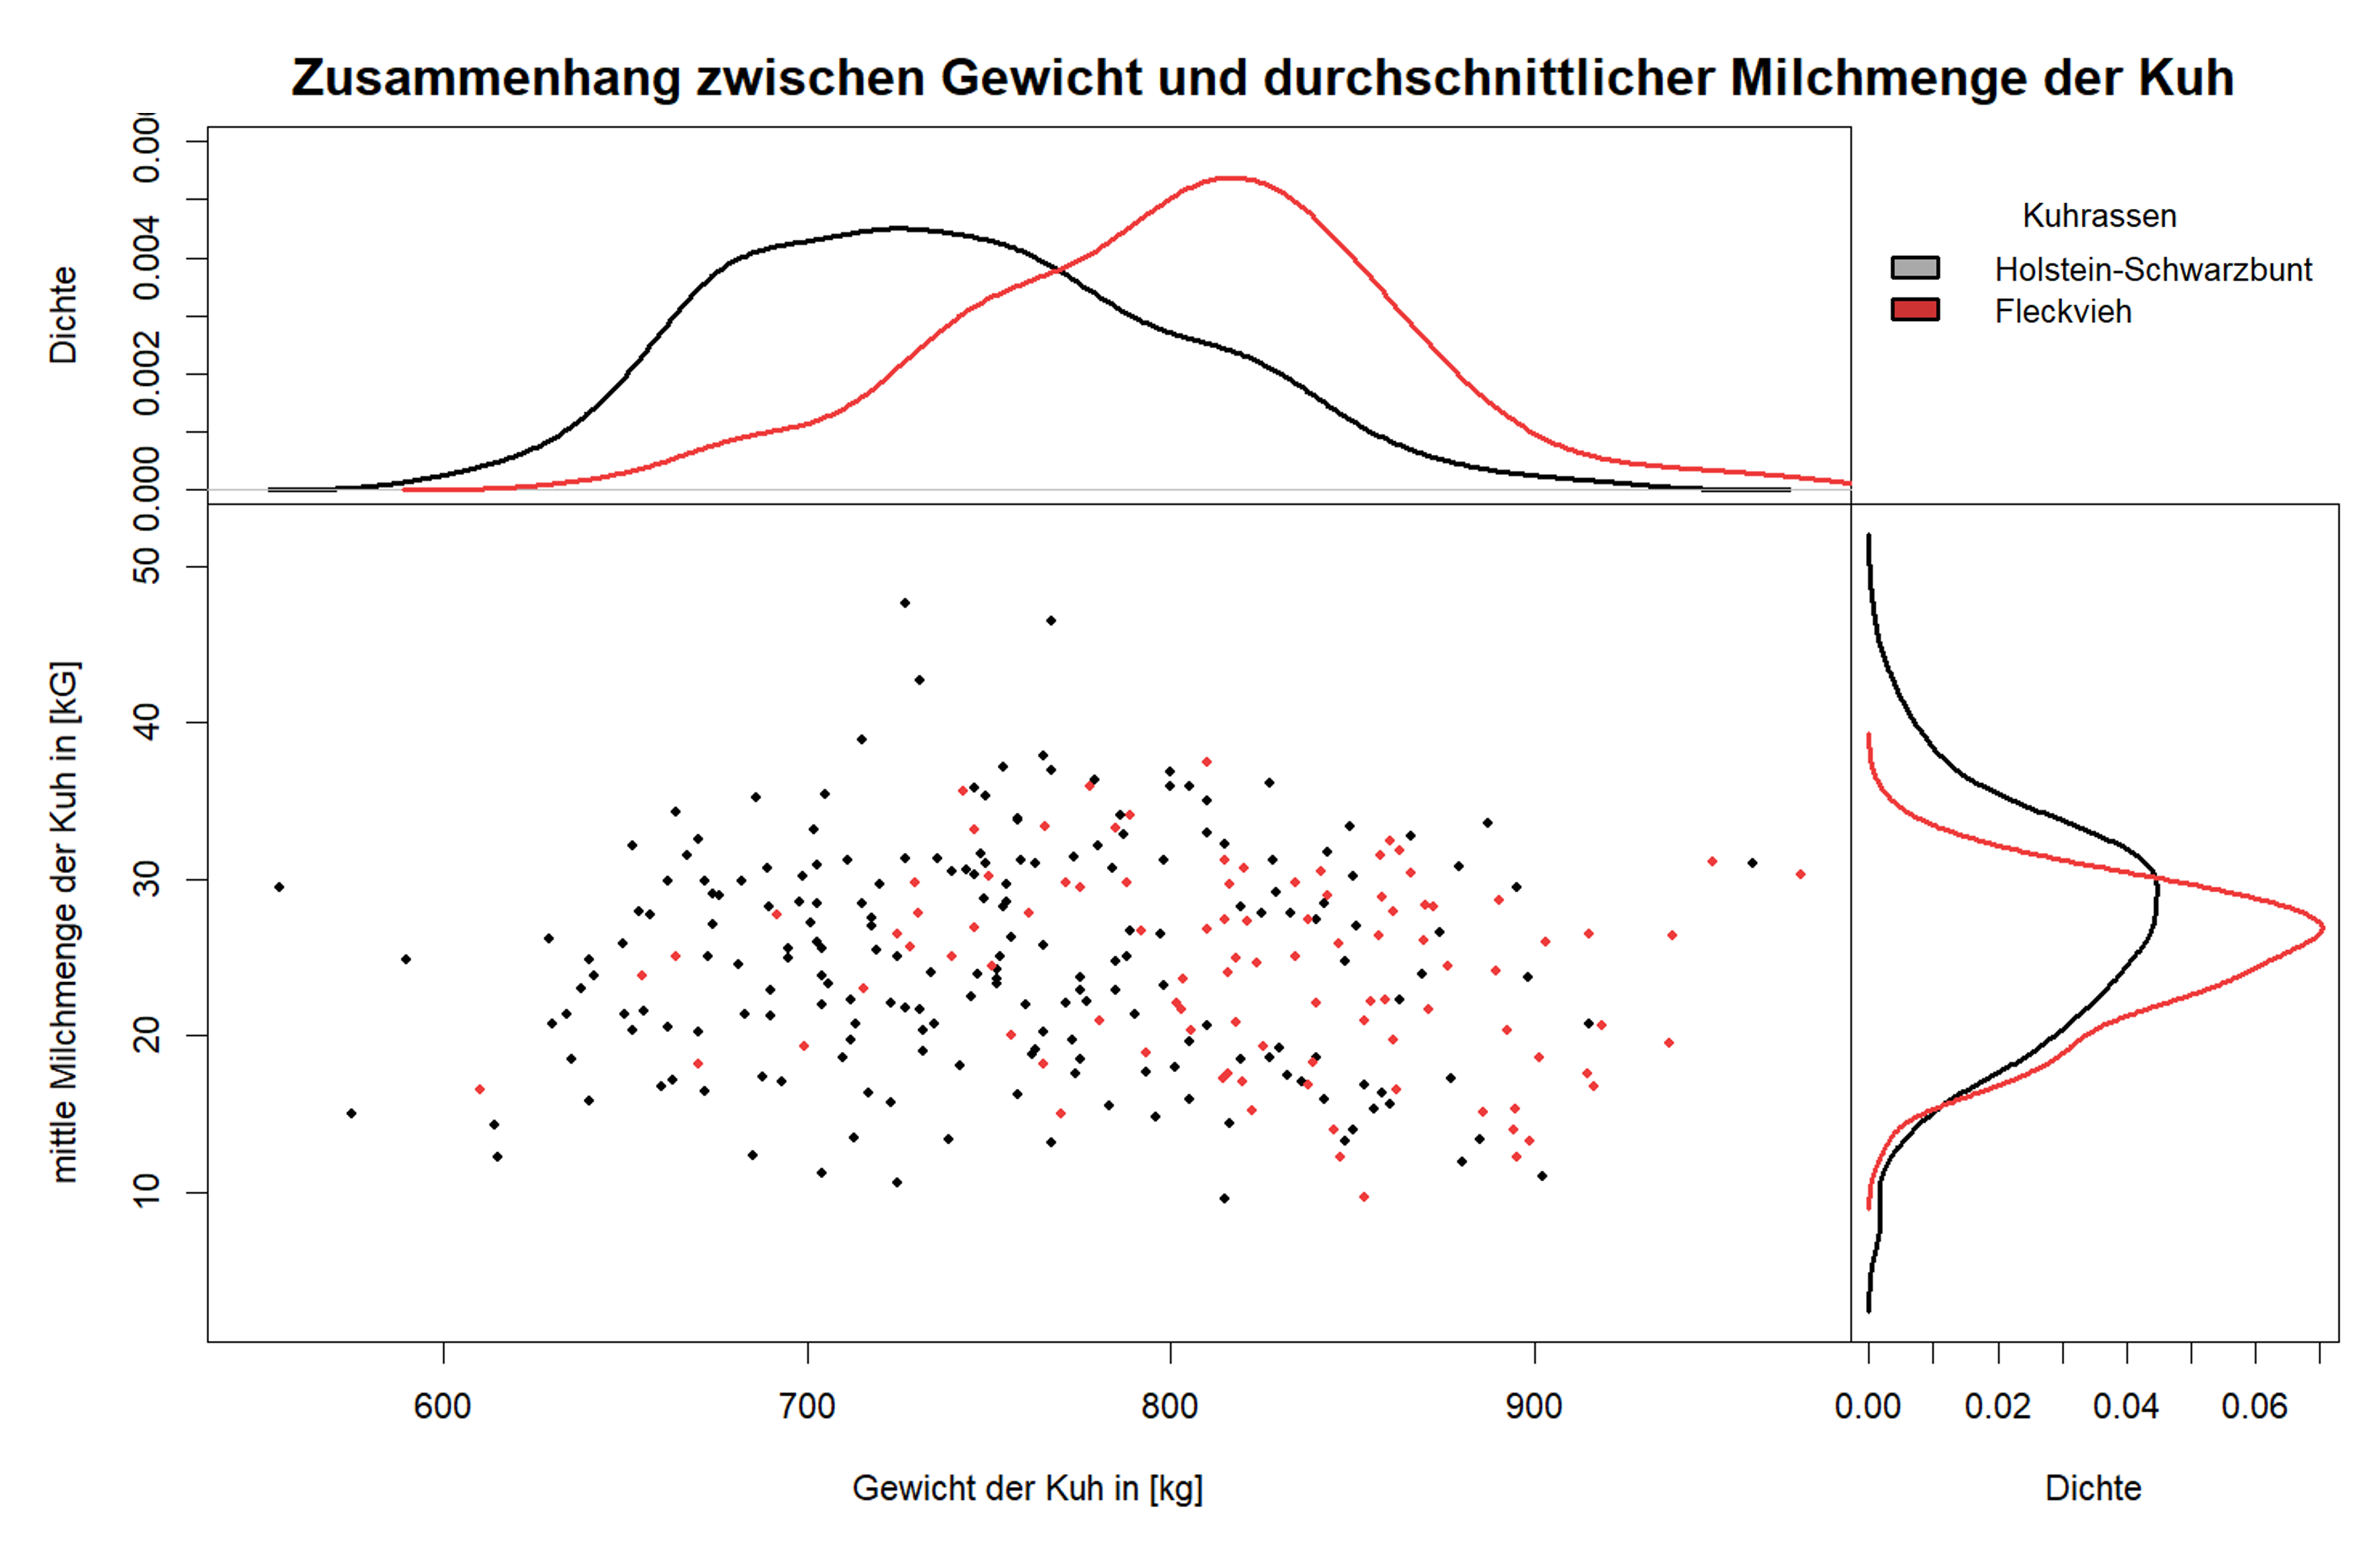
\includegraphics[width=1\textwidth]{Scatter und Kerndichte Milchmenge~Gewicht.png}
			\vspace{-0.6cm}
			\caption{Scatterplot und Kerndichten zur Gegenüberstellung der Milchmenge und des Gewichts}
		\end{figure}
	\end{frame}

    	\section{Milchmenge je Farm}
	\begin{frame}
		\frametitle{Milchmenge je Farm}
		\begin{figure}[h]
			\centering
			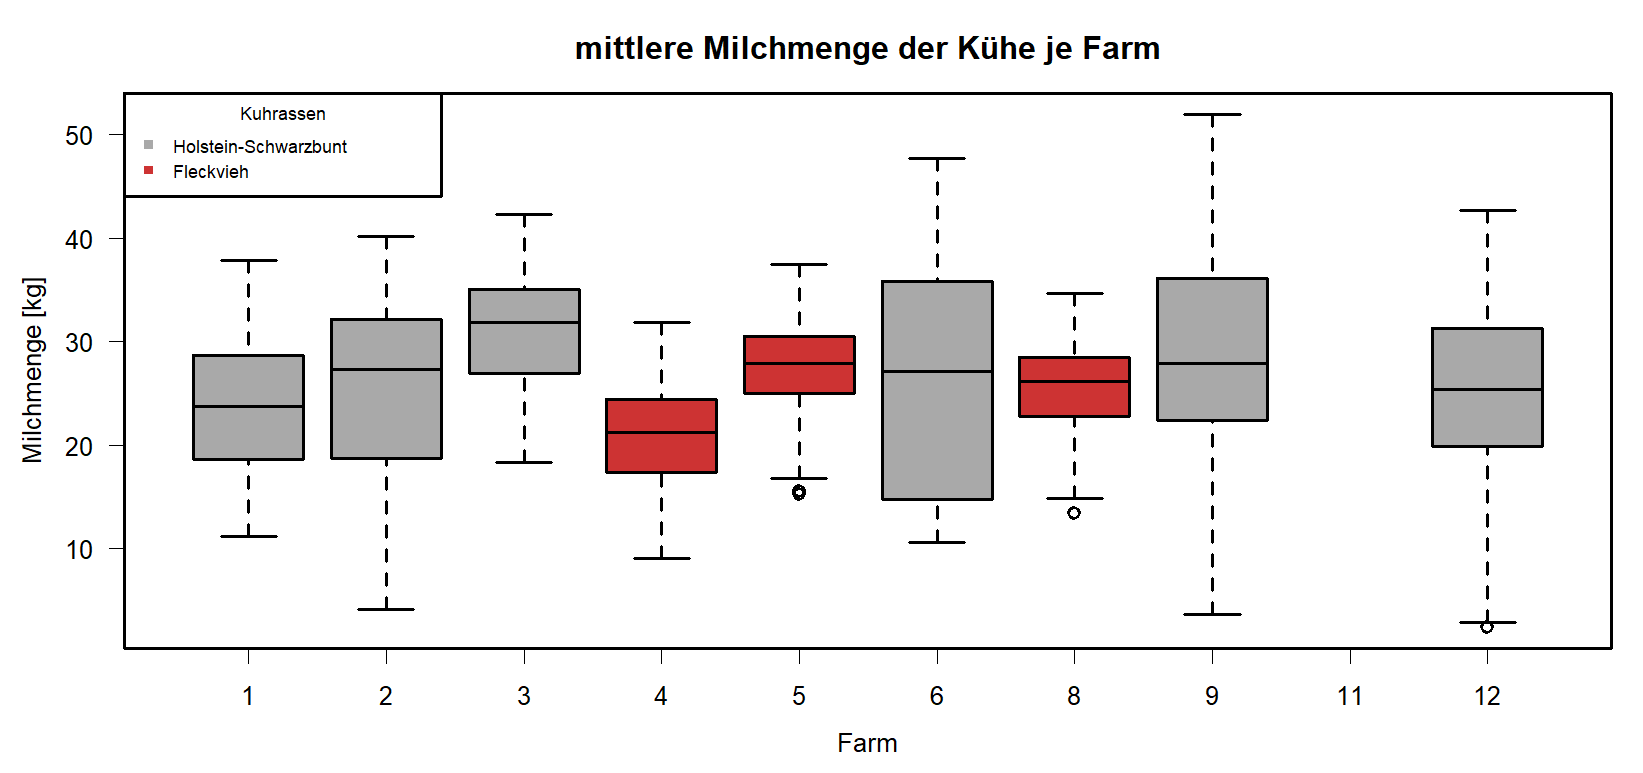
\includegraphics[width=1\textwidth]{Boxplot Milch~Farm.png}
			\vspace{-0.6cm}
			\caption{Boxplots zur mittleren durchschnittlichen Milchmenge je Farm}
		\end{figure}
	\end{frame}
\begin{frame}
	\section{Literaturverzeichnis}
	\frametitle{Literaturverzeichnis}
	Sarkar D (2008). \_Lattice: Multivariate Data Visualization with R\_.
	Springer, New York. ISBN 978-0-387-75968-5,
	<http://lmdvr.r-forge.r-project.org>.
\end{frame}
\end{document}
